% gxu-funktioner-og-ligninger.tex
% GXU worksheet, 8.-9. klasse (MULTI 7-9, kap. 6 + kap. 3)
% 1 opgave med 4 delopgaver, fokus på lineære + 1 delopgave om potens
% Struktur: Regel -> Eksempel -> Opgave 1.1 ... 1.4 -> Appendix med facit.
% INGEN skrive-linjer, INGEN navn/dato-felter.

\documentclass[11pt,a4paper]{article}

\usepackage[danish]{babel}
\usepackage[T1]{fontenc}
\usepackage[utf8]{inputenc}
\usepackage{icomma}
\usepackage{amsmath, amssymb, mathtools}
\usepackage{booktabs, enumitem, graphicx, xcolor, environ}
\usepackage{tikz}
\usetikzlibrary{arrows.meta, calc, positioning}
\usepackage{float}
\usepackage[hidelinks]{hyperref}
\usepackage[capitalise,nameinlink]{cleveref}
\usepackage[most]{tcolorbox}
\tcbuselibrary{skins, breakable}
\usepackage{fancyhdr}
\usepackage{geometry}
\geometry{a4paper, margin=2.5cm}
\usepackage{parskip}

% --- GXU palette (samme som GXU-MISC) ---
\definecolor{gxu-paper}{HTML}{F7F9FB}
\definecolor{gxu-ink}{HTML}{1A1F2B}
\definecolor{gxu-inksoft}{HTML}{4A5568}
\definecolor{gxu-accent}{HTML}{58C4DD}
\definecolor{gxu-purple}{HTML}{7C5CFC}
\definecolor{boxframe}{HTML}{CBD5E0}

% --- facit-flag (flip til false for elev-udgave) ---
\newif\ifshowanswers
\showanswerstrue

% --- box-styles (prompt / solution / definition / kompetence-chip) ---
\newtcolorbox{prompt}{
  colback=gxu-paper, colframe=gxu-accent, boxrule=0.5pt, arc=4pt,
  left=8pt, right=8pt, top=6pt, bottom=6pt,
  fonttitle=\sffamily\small\bfseries, title=Opgave
}
\newtcolorbox{solution}{
  colback=gxu-accent!8, colframe=gxu-accent, boxrule=0.5pt, arc=4pt,
  left=8pt, right=8pt, top=6pt, bottom=6pt,
  fonttitle=\sffamily\small\bfseries, title=Facit
}
\NewEnviron{solutionc}{\ifshowanswers\begin{solution}\BODY\end{solution}\fi}
\newtcolorbox{regelbox}{
  colback=gxu-paper, colframe=gxu-accent, boxrule=0.6pt, arc=4pt,
  left=8pt, right=8pt, top=6pt, bottom=6pt
}

\newcommand{\kompetence}[1]{%
  \tcbset{mychip/.style={colback=gxu-accent!15,colframe=gxu-accent,boxrule=0.4pt,arc=10pt,left=6pt,right=6pt,top=3pt,bottom=3pt,fontupper=\sffamily\small}}%
  \begin{tcolorbox}[mychip]#1\end{tcolorbox}\vspace{-4pt}%
}

\makeatletter
\newcommand{\eq}[2]{\begin{equation}#2\tag{#1}\end{equation}}
\makeatother
\newcommand{\note}[1]{{\small\color{gxu-inksoft}\textit{#1}}\par}

% --- header / footer ---
\pagestyle{fancy}
\fancyhf{}
\fancyhead[L]{\sffamily\small\color{gxu-inksoft}GXU -- Matematik}
\fancyhead[R]{\sffamily\small\color{gxu-inksoft}Funktioner og ligninger}
\fancyfoot[C]{\sffamily\small\color{gxu-inksoft}\thepage}
\renewcommand{\headrulewidth}{0.0pt}

% --- sektion-stil (accent på section-overskrift, samme som GXU-MISC) ---
\usepackage{titlesec}
\titleformat{\section}{\Large\bfseries\color{gxu-accent}}{\thesection}{0.6em}{}
\titleformat{\subsection}{\large\bfseries\color{gxu-accent}}{\thesubsection}{0.6em}{}
\titleformat{\subsubsection}{\normalsize\bfseries\color{gxu-ink}}{\thesubsubsection}{0.6em}{}
\titlespacing*{\section}{0pt}{1.4em}{0.6em}
\titlespacing*{\subsection}{0pt}{1.0em}{0.4em}

\begin{document}

% ============================================================
% Titel
% ============================================================
\begin{center}
  {\Large\bfseries Funktioner og ligninger}\\[2pt]
  {\color{gxu-inksoft}\large Træningsopgavesæt}\\[6pt]
  {\color{gxu-inksoft}\small 8.--9. klasse \quad -- \quad MULTI 7-9, kap.\ 6 og 3}
\end{center}

\vspace{6pt}
\hrule height 0.4pt
\vspace{10pt}

\noindent
Hver sektion starter med en kort regel og et udregnet eksempel --- så kan du
løse de følgende opgaver på samme måde. Facit ligger bagerst i appendix.

% ============================================================
% Lineære funktioner
% ============================================================
\section{Lineære funktioner}

\kompetence{Repraesentation} \kompetence{Modellering}

\noindent
En lineær funktion har formen
\eq{1.1}{f(x) = a\,x + b}
hvor $a$ er hældningen (hvor stejl linjen er) og $b$ er skæringen med $y$-aksen
(hvor linjen krydser $y$-aksen, altså $f(0)$).

\begin{figure}[h]
\centering
\begin{tikzpicture}[>=Stealth, scale=0.9, line cap=round, line join=round]
  % koordinatsystem
  \draw[->] (-2.5,0) -- (5.5,0) node[below] {$x$};
  \draw[->] (0,-3.5) -- (0,11.5) node[left] {$y$};
  % linjen f(x) = 2x+1
  \draw[very thick, gxu-accent] (-2,-3) -- (5,11);
  % punkter
  \foreach \x/\y in {-2/-3,-1/-1,0/1,1/3,2/5,3/7,4/9,5/11}{
    \fill[gxu-ink] (\x,\y) circle (1.6pt);
  }
  % skæringspunkt med y-aksen
  \draw[->, thick, gxu-inksoft] (0.55,0.55) -- (0.05,0.95);
  \node[anchor=west, gxu-inksoft] at (0.7,0.7) {$f(0)=b=1$};
  % et punkt fremhævet
  \draw[->, thick, gxu-inksoft] (2.4,5.4) -- (2.05,5.05);
  \node[anchor=west, gxu-inksoft] at (2.5,5.5) {$(2,5)$};
\end{tikzpicture}
\caption{Lineær funktion $f(x)=2x+1$ med hældning $a=2$ og $y$-skæring $b=1$.}
\label{fig:linear}
\end{figure}

\note{Hældningen $a$ er ændringen i $f(x)$ når $x$ vokser med $1$.}

\subsection*{Eksempel --- aflæs $f(2)$ og $f(5)$ på grafen}

På grafen ovenfor ser vi, at linjen passerer $(0,1)$ og $(2,5)$. Altså er
$f(2)=5$ og $f(5)=11$ (linjen går 2 op for hver 1 frem).

\subsection*{Eksempel --- find $a$ og $b$ for en linje}

Linjen $g(x) = -3x + 4$ har $a=-3$ (hældning, negativ fordi den falder)
og $b=4$ ($y$-skæring, fordi $g(0)=4$).

\vspace{8pt}
\begin{regelbox}
\textbf{Regel --- lineær funktion:} $f(x)=ax+b$. Hældning $a$, $y$-skæring $b$.
Grafen er en ret linje.
\end{regelbox}

% ============================================================
% Førstegradsligninger
% ============================================================
\section{Førstegradsligninger}

\kompetence{Tankegang} \kompetence{Regning}

\noindent
At løse en ligning betyder at finde den værdi af $x$ der gør begge sider lige
store. Vi bruger \emph{ligevægts-princippet}: hvad du gør på den ene side af
lighedstegnet, skal du også gøre på den anden side.

\begin{regelbox}
\textbf{Regel --- løs $ax+b=c$:} Træk $b$ fra på begge sider, divider med
$a$ på begge sider. Tjek altid til sidst ved at indsætte.
\end{regelbox}

\subsection*{Eksempel --- løs $2x + 1 = 7$}
\begin{align*}
  2x + 1 &= 7    &&\text{træk $1$ fra}\\
  2x     &= 6    &&\text{divider med $2$}\\
  x      &= 3
\end{align*}
Tjek: $2\cdot 3 + 1 = 7$ \checkmark.

\subsection*{Eksempel --- løs $-3x + 4 = 13$}
\begin{align*}
  -3x + 4 &= 13   &&\text{træk $4$ fra}\\
  -3x     &= 9    &&\text{divider med $-3$}\\
  x       &= -3
\end{align*}
Tjek: $-3\cdot(-3) + 4 = 9 + 4 = 13$ \checkmark.

\note{Hvis du dividerer med et negativt tal, skifter $x$ fortegn.}

% ============================================================
% Ligningssystem
% ============================================================
\section{Ligningssystemer (to linjer)}

\kompetence{Modellering} \kompetence{Repraesentation}

\noindent
Et ligningssystem består af to (eller flere) ligninger med to (eller flere)
ubekendte. Vi løser det ved at finde det punkt $(x,y)$ der opfylder alle
ligninger på én gang.

\begin{regelbox}
\textbf{Regel --- løs grafisk:} Tegn begge linjer i samme koordinatsystem.
Løsningen er der hvor de skærer hinanden.

\textbf{Regel --- løs algebraisk:} Sæt de to udtryk for $y$ lig hinanden,
løs for $x$, og find så $y$ ved at indsætte i en af ligningerne.
\end{regelbox}

\subsection*{Eksempel --- løs $y = 2x+1$ og $y = -x+7$}

Sæt højre sider lig hinanden:
\begin{align*}
  2x + 1   &= -x + 7   &&\text{læg $x$ til}\\
  3x + 1   &= 7        &&\text{træk $1$ fra}\\
  3x       &= 6        &&\text{divider med $3$}\\
  x        &= 2
\end{align*}
Indsæt $x=2$ i første ligning: $y = 2\cdot 2 + 1 = 5$.\\
Løsning: $(x,y) = (2,5)$. Tjek i anden ligning: $-2 + 7 = 5$ \checkmark.

\begin{figure}[h]
\centering
\begin{tikzpicture}[>=Stealth, scale=0.8, line cap=round, line join=round]
  % koordinatsystem
  \draw[->] (-1.5,0) -- (8.5,0) node[below] {$x$};
  \draw[->] (0,-2.5) -- (0,15.5) node[left] {$y$};
  % linjer
  \draw[very thick, gxu-accent] (-1,-1) -- (7,15);
  \node[gxu-inksoft] at (6.5,14.2) {\small (I) $y=2x+1$};
  \draw[very thick, gxu-purple] (-1,8) -- (8,-1)
    node[pos=0.95, above left=2pt, gxu-inksoft] {\small (II) $y=-x+7$};
  % skæringspunkt
  \fill[gxu-ink] (2,5) circle (2.2pt);
  \draw[->, thick, gxu-inksoft] (0.5,7.5) -- (1.9,5.2);
  \node[anchor=south west, gxu-inksoft] at (0.6,7.5) {$(2,5)$};
\end{tikzpicture}
\caption{To linjer skærer i $(2,5)$ -- den grafiske løsning på
         $y=2x+1$ og $y=-x+7$.}
\label{fig:system}
\end{figure}

% ============================================================
% Potensfunktion (bonus)
% ===========================================================
\section{Potensfunktioner (bonus)}

\kompetence{Repraesentation} \kompetence{Modellering}

\noindent
En potensfunktion har formen
\eq{4.1}{y = b \cdot x^{a}}
hvor $b$ og $a$ er konstanter. Når $a=1$ er funktionen lineær. Når
$a \neq 1$ er den \emph{ikke-lineær} --- grafen bøjer af.

\begin{regelbox}
\textbf{Regel --- potens:} $y = b\,x^{a}$. Hvis $a>1$ vokser funktionen
hurtigere end en lineær funktion for store $x$.
\end{regelbox}

\subsection*{Eksempel --- $y = 3\,x^{1{,}5}$}

\noindent
\begin{minipage}[t]{0.45\textwidth}
\centering
\renewcommand{\arraystretch}{1.15}
\begin{tabular}{lcccccc}
\toprule
$x$ & $0$ & $1$ & $2$ & $3$ & $4$ & $5$ \\
\midrule
$y = 3\,x^{1{,}5}$ & $0$ & $3$ & $\approx 8{,}49$ & $\approx 15{,}59$ & $24$ & $\approx 33{,}54$ \\
$y = 3x$           & $0$ & $3$ & $6$ & $9$ & $12$ & $15$ \\
\bottomrule
\end{tabular}

\vspace{4pt}
\footnotesize Ved $x=4$: potens dobbelt så stor ($24$ mod $12$).
\end{minipage}%
\hfill
\begin{minipage}[t]{0.5\textwidth}
\centering
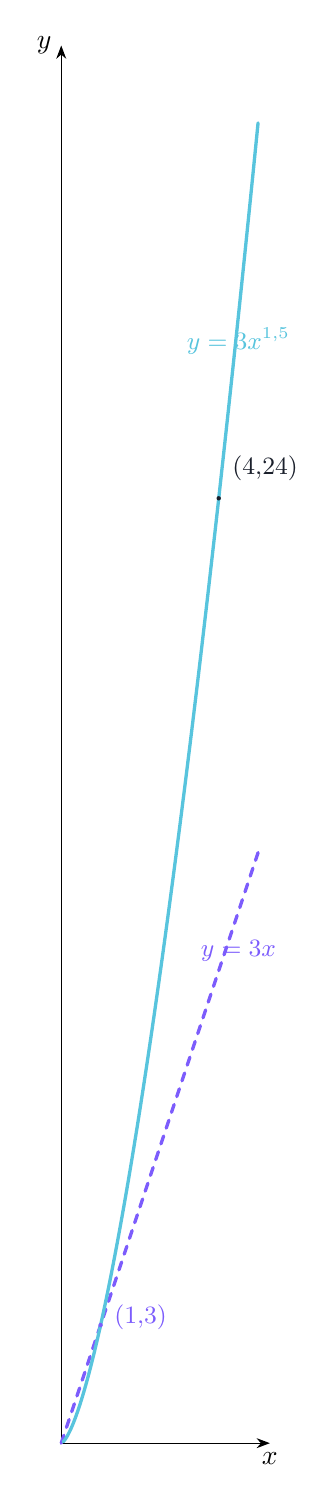
\begin{tikzpicture}[>=Stealth, scale=0.5, line cap=round, line join=round]
  \draw[->] (0,0) -- (5.3,0) node[below] {$x$};
  \draw[->] (0,0) -- (0,35.5) node[left] {$y$};
  \draw[very thick, dashed, gxu-purple] (0,0) -- (5,15);
  \node[gxu-purple] at (4.5,12.5) {\small $y=3x$};
  \draw[very thick, gxu-accent, smooth, samples=80, domain=0.05:5]
    plot (\x, {3*(\x^1.5)});
  \node[gxu-accent] at (4.5,28) {\small $y=3x^{1{,}5}$};
  \fill[gxu-purple] (1,3) circle (1.6pt);
  \node[gxu-purple, anchor=west] at (1.1,3.2) {\small $(1,3)$};
  \fill[gxu-ink] (4,24) circle (1.6pt);
  \node[gxu-ink, anchor=south west] at (4.1,24.2) {\small $(4,24)$};
\end{tikzpicture}
\end{minipage}

\vspace{4pt}
\noindent Potensen vokser hurtigere end den lineære: dobbelt så stor ved $x=4$,
mere end dobbelt ved $x=5$.

\note{Når $x=1$ giver enhver potens $y=b$ uanset eksponent --- derfor mødes
kurverne altid i $(1,b)$.}

% ============================================================
% Opgave 1: facit-løse opgaver
% ===========================================================
\section{Opgave 1 --- Løs selv}

\noindent
Brug eksemplerne ovenfor som skabelon. Facit bagerst.

\begin{prompt}
\textbf{1.1} \quad Løs ligningen $\,3x - 5 = 16$.
\end{prompt}

\begin{prompt}
\textbf{1.2} \quad Løs ligningen $\,-2x + 7 = 1$.
\end{prompt}

\begin{prompt}
\textbf{1.3} \quad Løs ligningssystemet
\begin{align*}
  y &= 3x - 2 \\
  y &= -x + 6
\end{align*}
\end{prompt}

\begin{prompt}
\textbf{1.4} \quad For potensfunktionen $y = 2 \cdot x^{1{,}5}$, udfyld en
tabel for $x=0,1,2,3,4$ og forklar med to tal hvorfor den vokser hurtigere
end den lineære $y = 2x$.
\end{prompt}

% ============================================================
% Appendix: facit
% ============================================================
\newpage
\section*{Appendix --- Facit}

\noindent\textbf{Ligninger}
\begin{itemize}[leftmargin=2em, itemsep=4pt]
  \item \textbf{1.1:} $3x-5=16 \Rightarrow 3x=21 \Rightarrow x=7$.\\
        Tjek: $3\cdot 7 - 5 = 21-5 = 16$ \checkmark.
  \item \textbf{1.2:} $-2x+7=1 \Rightarrow -2x=-6 \Rightarrow x=3$.\\
        Tjek: $-2\cdot 3 + 7 = -6+7 = 1$ \checkmark.
\end{itemize}

\noindent\textbf{Ligningssystem}
\begin{itemize}[leftmargin=2em, itemsep=4pt]
  \item \textbf{1.3:} Sæt højre sider lig: $3x-2 = -x+6 \Rightarrow 4x=8
        \Rightarrow x=2$. Indsæt: $y = 3\cdot 2 - 2 = 4$. Løsning $(2,4)$.\\
        Tjek (II): $-2+6 = 4$ \checkmark.
\end{itemize}

\noindent\textbf{Potensfunktion}
\begin{itemize}[leftmargin=2em, itemsep=4pt]
  \item \textbf{1.4:} $x=0 \Rightarrow y=0$; $x=1 \Rightarrow y=2$;
        $x=2 \Rightarrow y \approx 5{,}66$; $x=3 \Rightarrow y \approx 10{,}39$;
        $x=4 \Rightarrow y = 16$.\\
        Sammenligning: $2\cdot 4^{1{,}5} = 16$ mod $2\cdot 4 = 8$ (dobbelt);
        $2\cdot 5^{1{,}5} \approx 22{,}36$ mod $2\cdot 5 = 10$ (mere end
        dobbelt). Potensen vokser hurtigere.
\end{itemize}

\end{document}
